\begin{problem}{Гонка дронов}{стандартный ввод}{стандартный вывод}{2 секунды}{512 мегабайт}

В Иннополисе проводятся гонки дронов.

В гонке могут принять участие $n$ дронов, $i$-й дрон пролетает единицу расстояния за $t_i$ секунд.
Гонка проводится на прямой, на которой расположены $m$ ворот, пронумерованных от $1$ до $m$, $i$-е ворота находятся на расстоянии $s_i$ от стартовой позиции гонки.

В гонке примут участие первые $k$ дронов с номерами от $1$ до $k$. Величину $k$ судьи объявляют непосредственно перед гонкой, поэтому вам необходимо проанализировать гонку для всех $k$ от~$1$~до~$n$.

Гонка проводится следующим образом. 

Дроны начинают движение из точки $0$ в сторону ворот, каждый со своей скоростью. У каждого дрона есть \textit{точка восстановления} "--- последние ворота, в которых он выполнял \textit{сохранение позиции}. Изначально точка восстановления каждого дрона "--- точка $0$. Дроны каждый раз начинают двигаться из своих точек восстановления и продолжают движение, пока один или несколько дронов не оказываются в точке, где расположены ворота (возможно, различные для разных дронов). В этот момент среди всех дронов, которые оказались в каких-либо воротах, выбирается дрон с наименьшим номером. Для этого дрона производится сохранение позиции, его точка восстановления переносится в его текущую позицию. Остальные дроны мгновенно телепортируются в свои точки восстановления. После этого гонка продолжается таким же образом. 

Как только дрон сохраняет позицию в последних воротах с номером $m$, он финиширует. Не финишировавшие пока дроны, как обычно, телепортируются в свои точки восстановления и продолжают гонку. Когда все дроны финишируют, гонка завершается.

Телепортация "--- очень энергоемкий процесс. Для подготовки к гонке необходимо понять, сколько суммарно телепортаций совершат все дроны до её завершения. Обозначим как $c_k$ суммарное число телепортаций, которое совершат все дроны, если в гонке будут участвовать первые $k$ дронов. Найдите значения $c_1, c_2, \ldots, c_n$.

\InputFile
В первой строке даны два целых числа $n$ и $m$ "--- количество дронов и ворот, соответственно ($2 \le n \le 150\,000$, $1 \le m \le 150\,000$).

Во второй строке даны $n$ положительных целых чисел $t_1, t_2,...,t_n$, где $t_i$ "--- количество секунд, за которое $i$-й дрон пролетает единицу расстояния ($1 \le t_i \le 10^9$).

В третьей строке даны $m$ положительных целых чисел $s_1, s_2,...,s_m$, где $s_i$ "--- позиция $i$-х ворот на прямой ($1 \le s_1 < s_2 < \ldots < s_m \le 150\,000$).

\OutputFile
Выведите $n$ целых чисел $c_1, c_2, \ldots, c_n$.

\newpage
\Scoring
\begin{center}
\begingroup
\unskip
\renewcommand{\arraystretch}{1.5}
\begin{tabular}{|c|c|c|c|c|c|c|}
\hline
& & \multicolumn{4}{c|}{Ограничения} & \\
\cline{3-6}
\raisebox{2.25ex}[0cm][0cm]{Подз.}
& \raisebox{2.25ex}[0cm][0cm]{Баллы}
& $n$ & $m$ & $t_i, s_i$ & Доп. ограничения 
& \raisebox{2.25ex}[0cm][0cm]{\parbox{2cm}{\centering Необх. подзадачи}}
\\
\hline
1 & 5 & $n = 2$ & $m \le 50$ & $t_i,s_i \le 100\,000$ & & \\
\hline
2 & 7 & $n \le 50$ & $m \le 50$ & $t_i,s_i \le 100\,000$ & & У, 1 \\
\hline
3 & 13 & $n \le 1000$ & $m \le 5$ & $t_i,s_i \le 100\,000$ & & У \\
\hline
4 & 9 & $n \le 100\,000$ & $m \le 100\,000$ & $t_i,s_i \le 100\,000$ & \parbox[c][1.5cm]{2.5cm}{\centering $s_{i+1} - s_i = s_1$\\ для всех $1 \le i < m$} &  \\
\hline
5 & 8 & $n \le 100\,000$ & $m \le 100\,000$ & $t_i,s_i \le 100\,000$ & все $t_i$ равны &  \\
\hline
6 & 10 & $n \le 100$ & $m \le 100\,000$ & $t_i,s_i \le 100\,000$ & & У, 1 -- 2  \\
\hline
7 & 5 & $n \le 100\,000$  & $m \le 100\,000$ & $t_i \le 2$, $s_i \le 100\,000$ & &  \\
\hline
8 & 7 & $n \le 100\,000$ & $m=2$ & $t_i,s_i \le 100\,000$ & & \\
\hline
9 & 6 & $n \le 10\,000$ & $m \le 100\,000$ & $t_i,s_i \le 100\,000$ & & У, 1 -- 3, 6  \\
\hline
10 & 6 & $n \le 50\,000$ &$m \le 100\,000$ & $t_i,s_i \le 100\,000$ & & У, 1 -- 3, 6, 9  \\
\hline
11 & 8 & $n \le 100\,000$ &$m \le 100\,000$ & $t_i,s_i \le 100\,000$ & & У, 1 -- 10  \\
\hline
12 & 8 & $n \le 100\,000$ & & & & У, 1 -- 11  \\
\hline
13 & 8 & \multicolumn{3}{c|}{без дополнительных ограничений} & & У, 1 -- 12  \\
\hline

\end{tabular}
\endgroup
\end{center}

\Examples

\begin{example}
\exmpfile{example.01}{example.01.a}%
\exmpfile{example.02}{example.02.a}%
\exmpfile{example.03}{example.03.a}%
\end{example}

\newpage
\Explanations
Рассмотрим первый пример. 

Если $k = 1$, то телепортаций не происходит.

Если $k=2$, то гонка происходит следующим образом. На рисунках показаны моменты, когда дроны оказываются в воротах и происходит телепортация.

\medskip
\begin{center}
\begin{tabular}{cc}
\renewcommand{\arraystretch}{2}
%>{\centering}p{5cm}
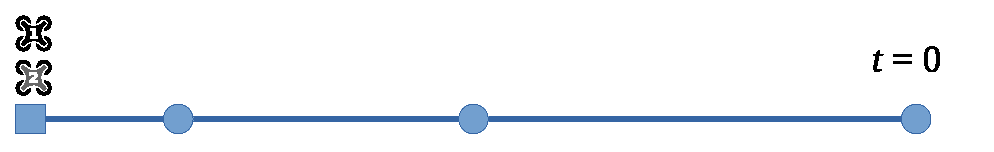
\includegraphics[scale=0.7]{sample-2-01.eps}\\[0.8cm]
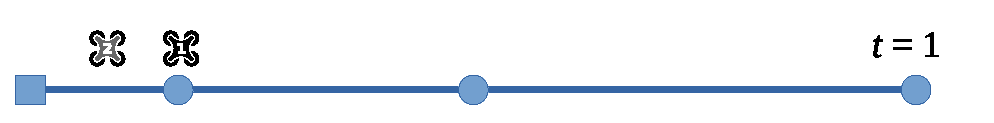
\includegraphics[scale=0.7]{sample-2-02.eps}\\[0.3cm]
\includegraphics[scale=0.7]{sample-2-03.eps}&{1 телепортация}\\[0.8cm]
\includegraphics[scale=0.7]{sample-2-04.eps}\\[0.3cm]
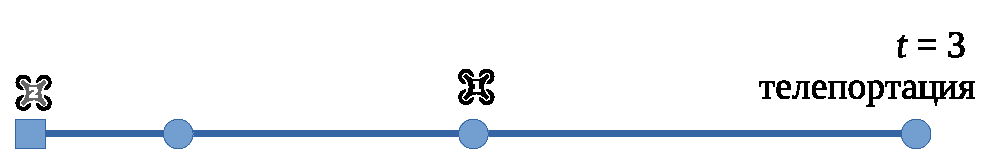
\includegraphics[scale=0.7]{sample-2-05.eps}&{+1 телепортация, итого 2}\\[0.8cm]
\includegraphics[scale=0.7]{sample-2-06.eps}\\[0.3cm]
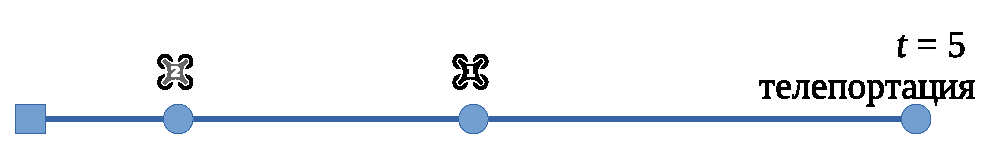
\includegraphics[scale=0.7]{sample-2-07.eps}&{+1 телепортация, итого 3}\\[0.8cm]
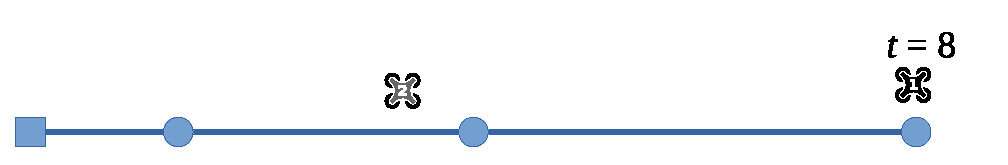
\includegraphics[scale=0.7]{sample-2-08.eps}&дрон 1 финишировал\\[0.3cm]
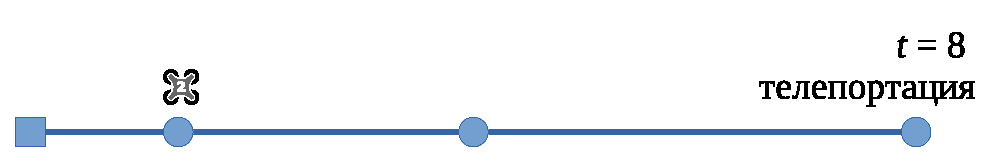
\includegraphics[scale=0.7]{sample-2-09.eps}&{+1 телепортация, итого 4}\\[0.8cm]
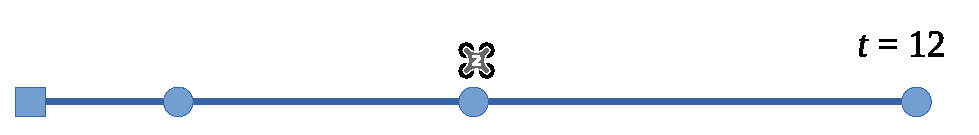
\includegraphics[scale=0.7]{sample-2-10.eps}\\[0.8cm]
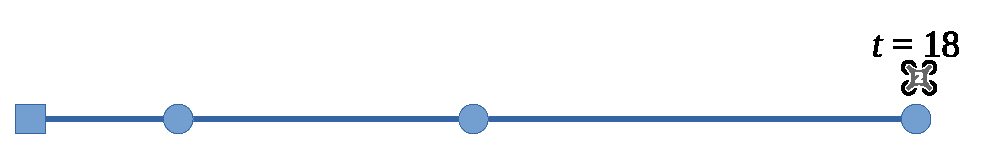
\includegraphics[scale=0.7]{sample-2-11.eps}&дрон 2 финишировал\\
\end{tabular}
\end{center}

Если $k=3$, то гонка происходит следующим образом. На рисунках показаны моменты, когда дроны оказываются в воротах и происходит телепортация.


\begin{center}
\begin{tabular}{cc}
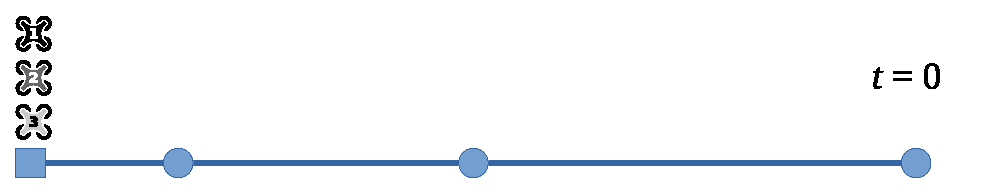
\includegraphics[scale=0.5]{sample-3-01.eps}\\[0.5cm]
\includegraphics[scale=0.5]{sample-3-02.eps}&
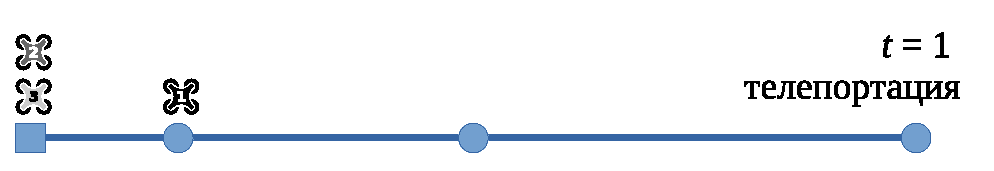
\includegraphics[scale=0.5]{sample-3-03.eps}\\
&2 телепортации\\[0.5cm]

\includegraphics[scale=0.5]{sample-3-04.eps}&
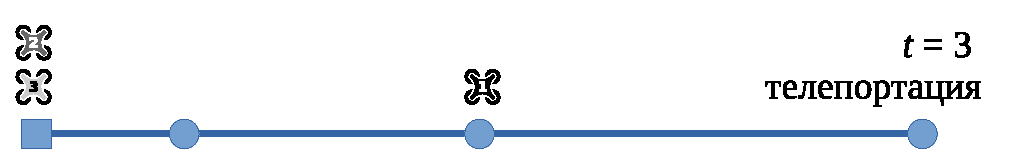
\includegraphics[scale=0.5]{sample-3-05.eps}\\
&+2 телепортации, итого 4\\[0.5cm]

\includegraphics[scale=0.5]{sample-3-06.eps}&
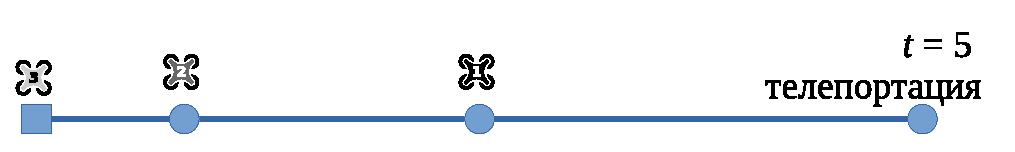
\includegraphics[scale=0.5]{sample-3-07.eps}\\
&+2 телепортации, итого 6\\[0.5cm]
\includegraphics[scale=0.5]{sample-3-08.eps}&
\includegraphics[scale=0.5]{sample-3-09.eps}\\
дрон 1 финишировал &+2 телепортации, итого 8\\[0.5cm]
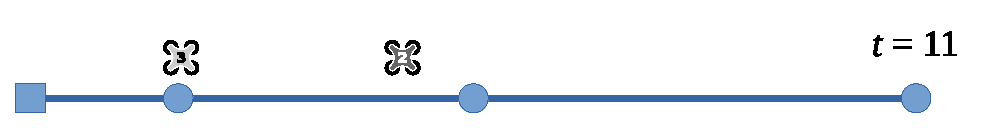
\includegraphics[scale=0.5]{sample-3-10.eps}&
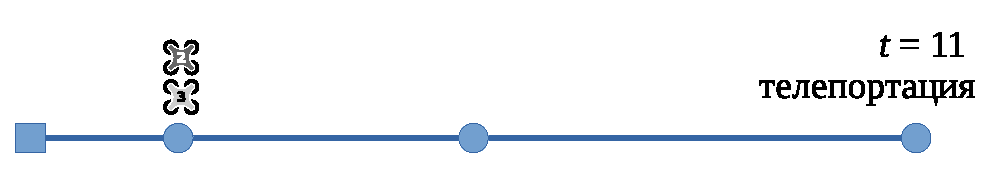
\includegraphics[scale=0.5]{sample-3-11.eps}\\
&+1 телепортация, итого 9\\[0.5cm]
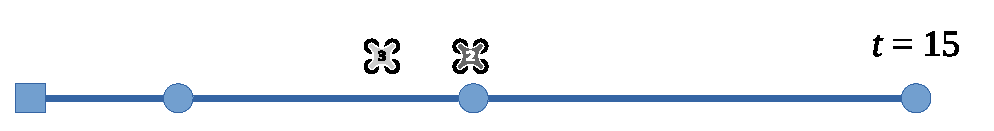
\includegraphics[scale=0.5]{sample-3-12.eps}&
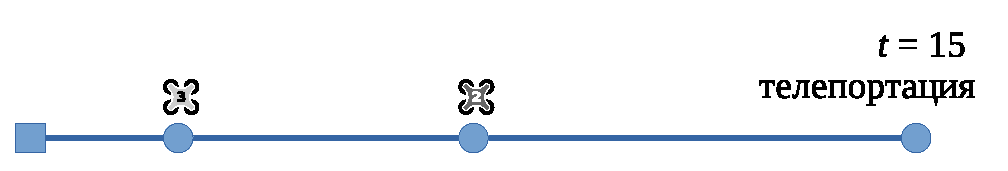
\includegraphics[scale=0.5]{sample-3-13.eps}\\
&+1 телепортация, итого 10\\[0.5cm]
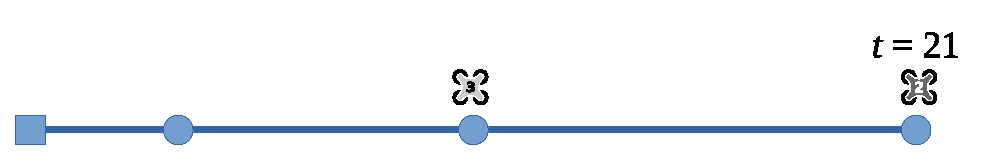
\includegraphics[scale=0.5]{sample-3-14.eps}&
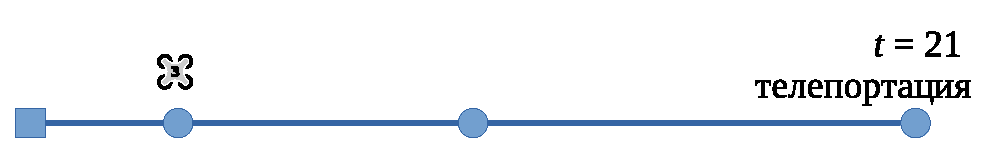
\includegraphics[scale=0.5]{sample-3-15.eps}\\
дрон 2 финишировал&+1 телепортация, итого 11\\[0.5cm]
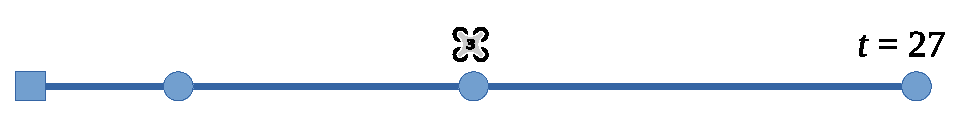
\includegraphics[scale=0.5]{sample-3-16.eps}&
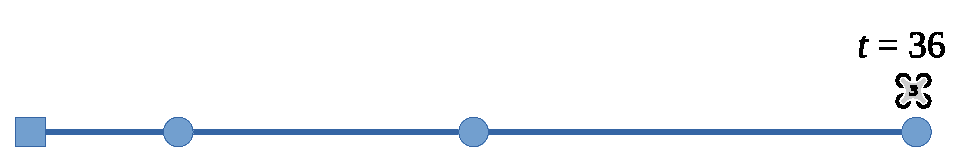
\includegraphics[scale=0.5]{sample-3-17.eps}\\
&дрон 3 финишировал\\
\end{tabular}
\end{center}




\end{problem}

